\section{Tree representation}

\subsection{Voting gmae}

    Three politicians are supposed to decide whether to raise their salaries or not. The vote is public and in sequence. They would prefer to receive a salary increase,
    yet they would also like to vote against it so as not to lose public support.
    Optimal result for each player: having salary increase while voting against it!
    Main features of the game:
1 The moves take place in sequence: the politicians vote one after the other
2 Every possible situation is known to the players: at any time they know the
whole past history, as well as the possible developments
3 The final outcome is determined by the majority of votes
This is an example of what is called a game with perfect information:
each player has knowledge about all the events that have previously occurred.
How can we represent such a game? And how can we solve it?
We may use a tree in which Each player’s vote is represented at a branch: YES on the left and NO on the right. 
Utilities are based on individual votes and possible final outcomes:
1= YES and no raise; 2= NO and no raise; 3= YES and raise; 4= N0 and raise
The tree in this case will become:
\begin{figure}[H]
    \centering
    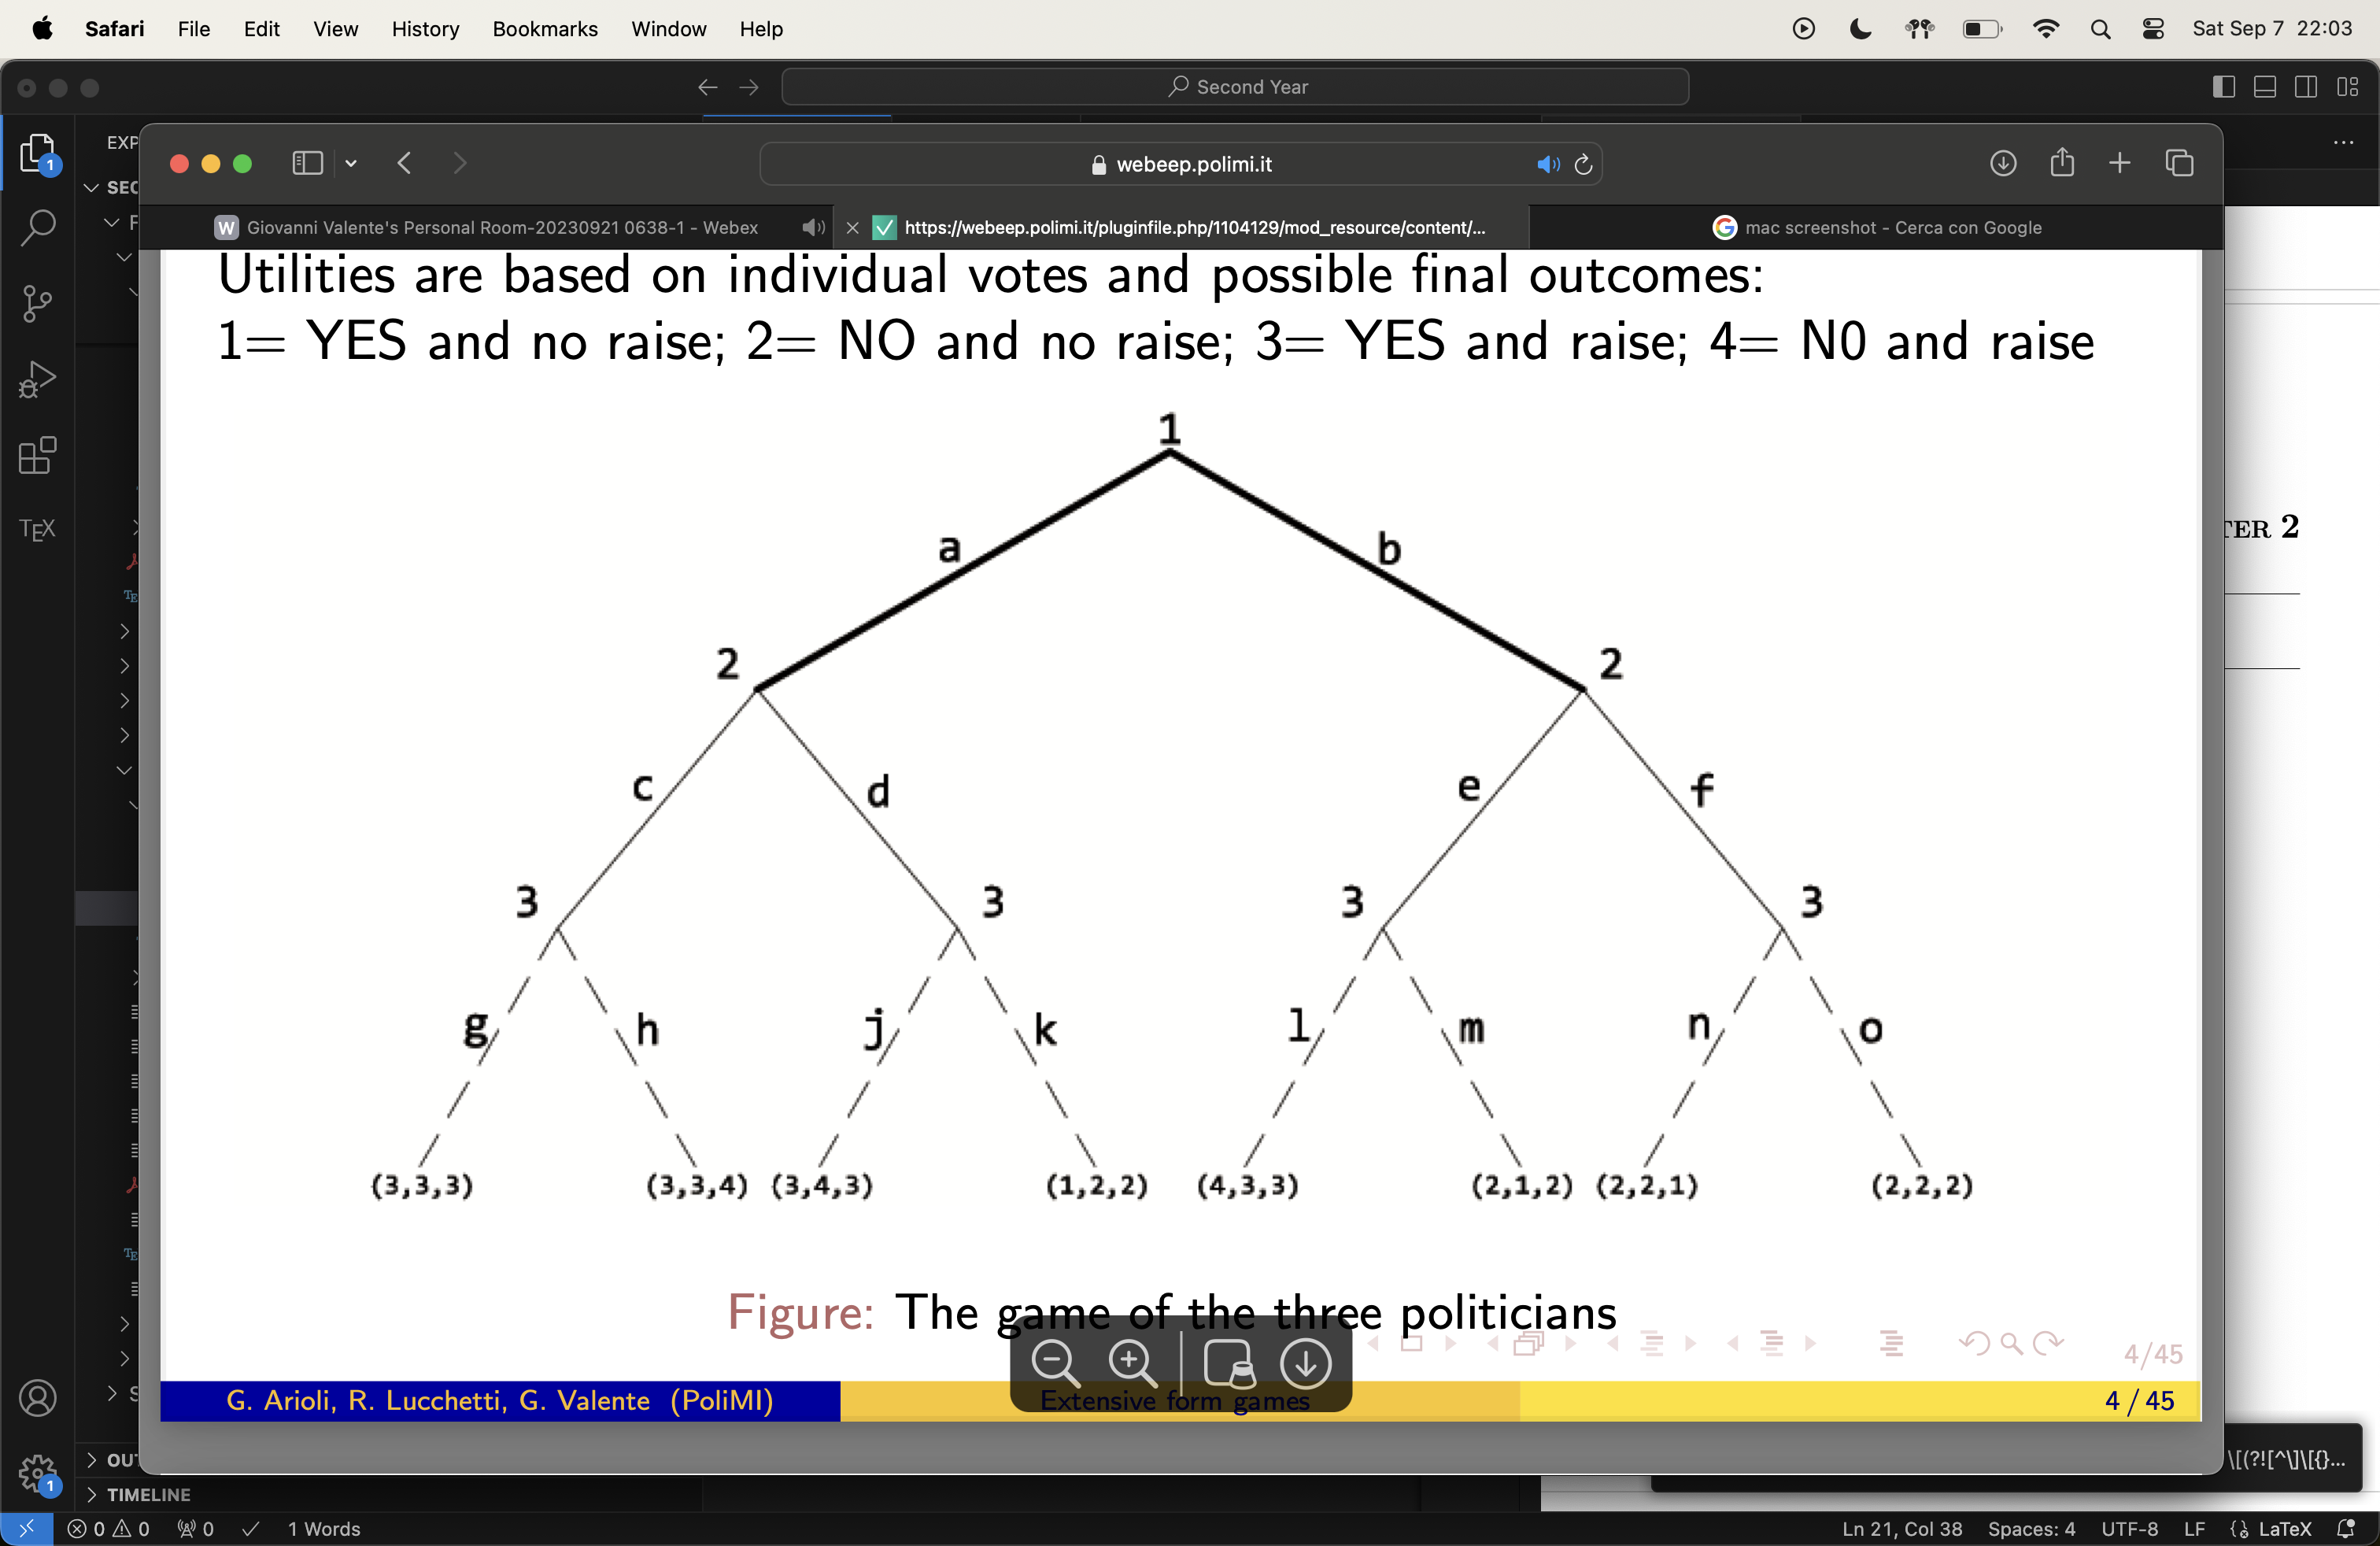
\includegraphics[width=0.75\linewidth]{images/tree.png}
    \caption{Voting game tree}
\end{figure}


\subsection{A game with chance}
Two players 1 and 2 must decide in sequence whether to play or not.
If both of them decide to play, then a coin is tossed (random component R): the first player wins with heads, whereas the second one with tails.
\begin{figure}[H]
    \centering
    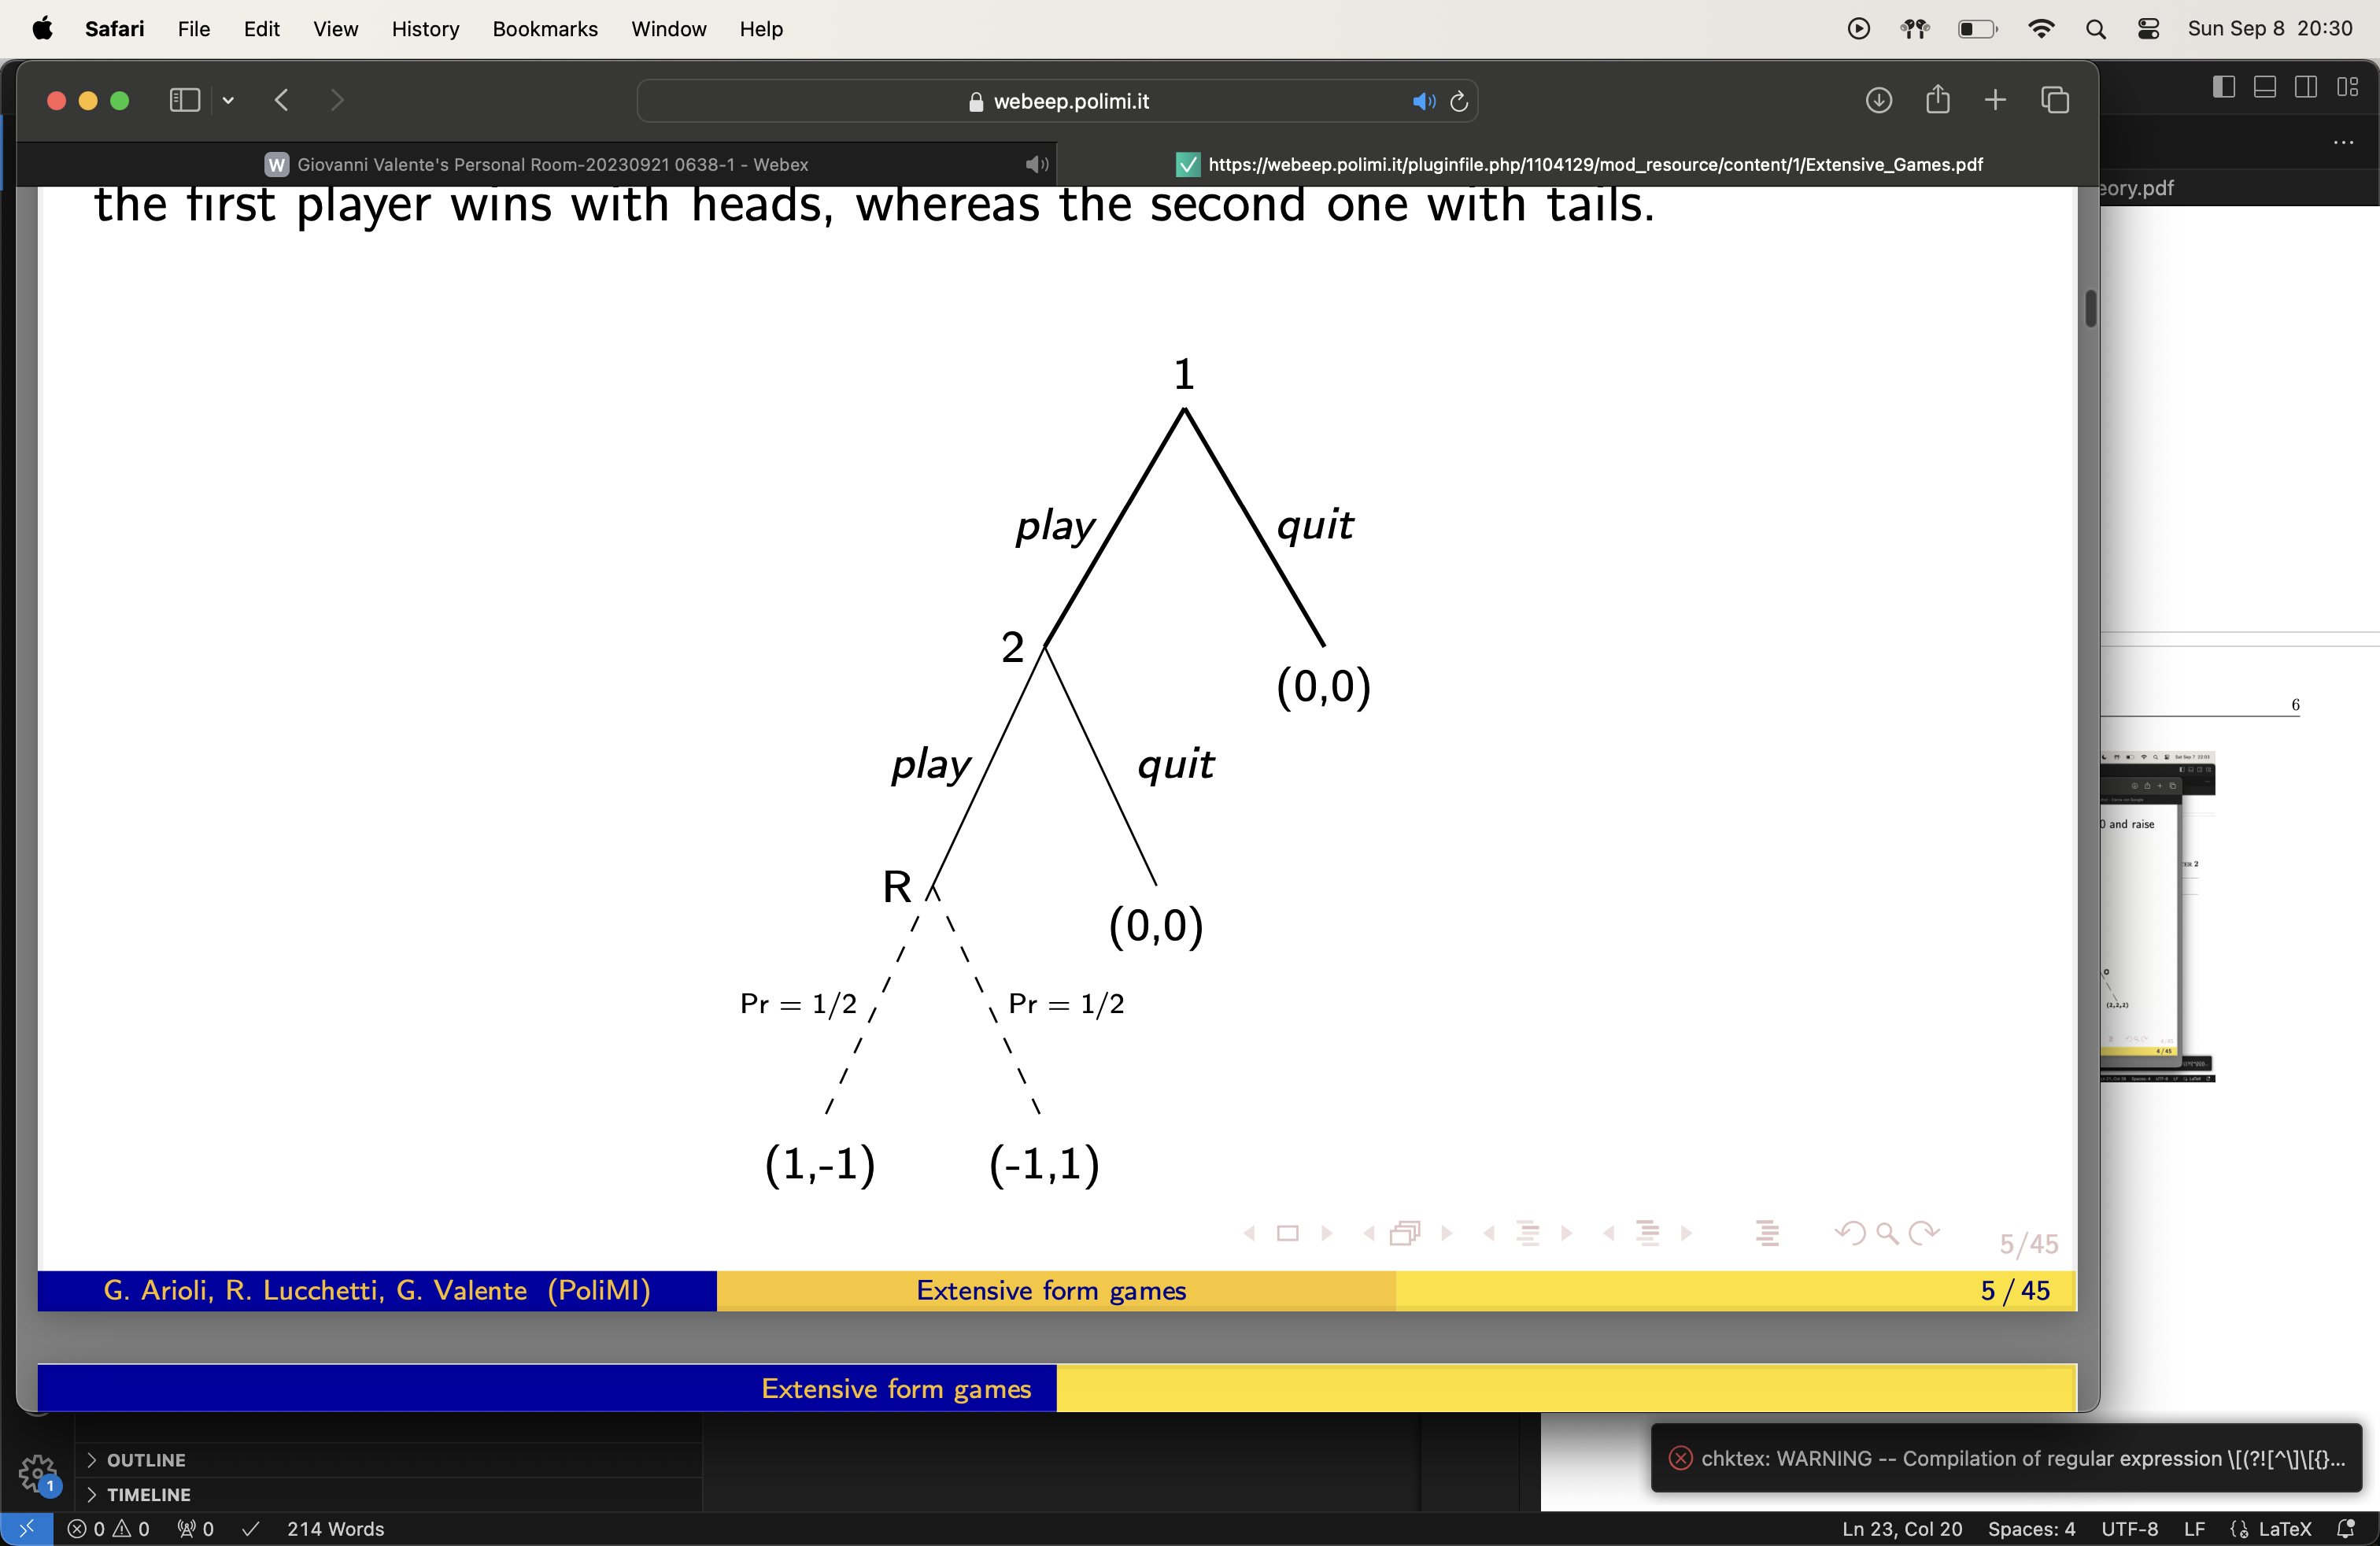
\includegraphics[width=0.75\linewidth]{images/tree1.png}
    \caption{Chance game tree}
\end{figure}

\subsection{Definitions}
\begin{definition}[\textit{Finite directed graph}]
    A finite directed graph is a pair $(V,E)$ where:
    \begin{itemize}
        \item $V$ is a finite set, called the set of vertices. 
        \item $E \subset V \times V$ is a set of ordered pairs of vertices called the set of the (directed) edges.
    \end{itemize}
\end{definition}
\begin{definition}[\textit{Path}]
    A path from a vertex $v_1$ to a vertex $v_{k+1}$ is a finite sequence of vertices-edges $v_1,e_1,v_2,\dots,v_k,e_k,v_{k+1}$ such that $e_i \neq e_j$ if $i \neq j$ and $e_j = (v_j,v_{j+1})$. 
    $k$ is called the length of the path. 
\end{definition}
\begin{definition}[\textit{Oriented graph}]
    An oriented graph is finite directed graph having no bidirected edges, that is for all $j,k$ at most one between $(v_j,v_k)$ and $(v_k,v_j)$ may be arrows of the graph.
\end{definition}
\begin{definition}[\textit{Tree}]
    A tree is a triple $(V,E,x_0)$ where $(V,E)$ is an oriented graph and $_x0$ is a vertex in $V$ such that there is a unique path from $x_0$ to $x$, where $x$ is any vertex in $V$. 
\end{definition}
\begin{definition}[\textit{Child}]
    A child of a vertex $v$ is any vertex $x$ such that $(v,x) \in E$. 
    A vertex is called a leaf if it has no children. 
    We say that the vertex $x$ follows the vertex $v$ if there is a path from $v$ to $x$.
\end{definition}


